%%%%%%%%%%%%%%%%%%%%%%%%%%%%%%%%%%%%%%%%%%%%%%%%%%%%%%%%%%%%%%%%%%%%%%%%%%%%%%%
% intro.tex: Introduction to the thesis
%%%%%%%%%%%%%%%%%%%%%%%%%%%%%%%%%%%%%%%%%%%%%%%%%%%%%%%%%%%%%%%%%%%%%%%%%%%%%%%%
\chapter{Verification of models}
\label{verifi_chapter}
%%%%%%%%%%%%%%%%%%%%%%%%%%%%%%%%%%%%%%%%%%%%%%%%%%%%%%%%%%%%%%%%%%%%%%%%%%%%%%%%

\section{Validation and verification of the VLE solvers and CFD solver} \label{App:vali}


    \subsection{Validation of the TP flash solver based on phase boundaries}
    The TP flash solver is validated by comparing the predictions with the experimental data of Somait and Kidnay \cite{somait1978liquid} in terms of the phase boundaries of \ce{CO2}/\ce{CH4} and \ce{CO2}/\ce{H2O} mixtures. As shown in Fig.~\ref{v1}, the model prediction agrees with the experimental data very well for both mixtures. In Fig.~\ref{v1} (a), we tested two different binary interaction parameters $k_{ij}$, and the results shows the effect of binary interaction parameters on the phase boundary. Appropriate values can improve the accuracy of phase boundary prediction.

    
    \begin{figure}[htbp]
        \centering
        \subfigure{
            %\begin{minipage}[t]{0.5\linewidth}
            \centering
            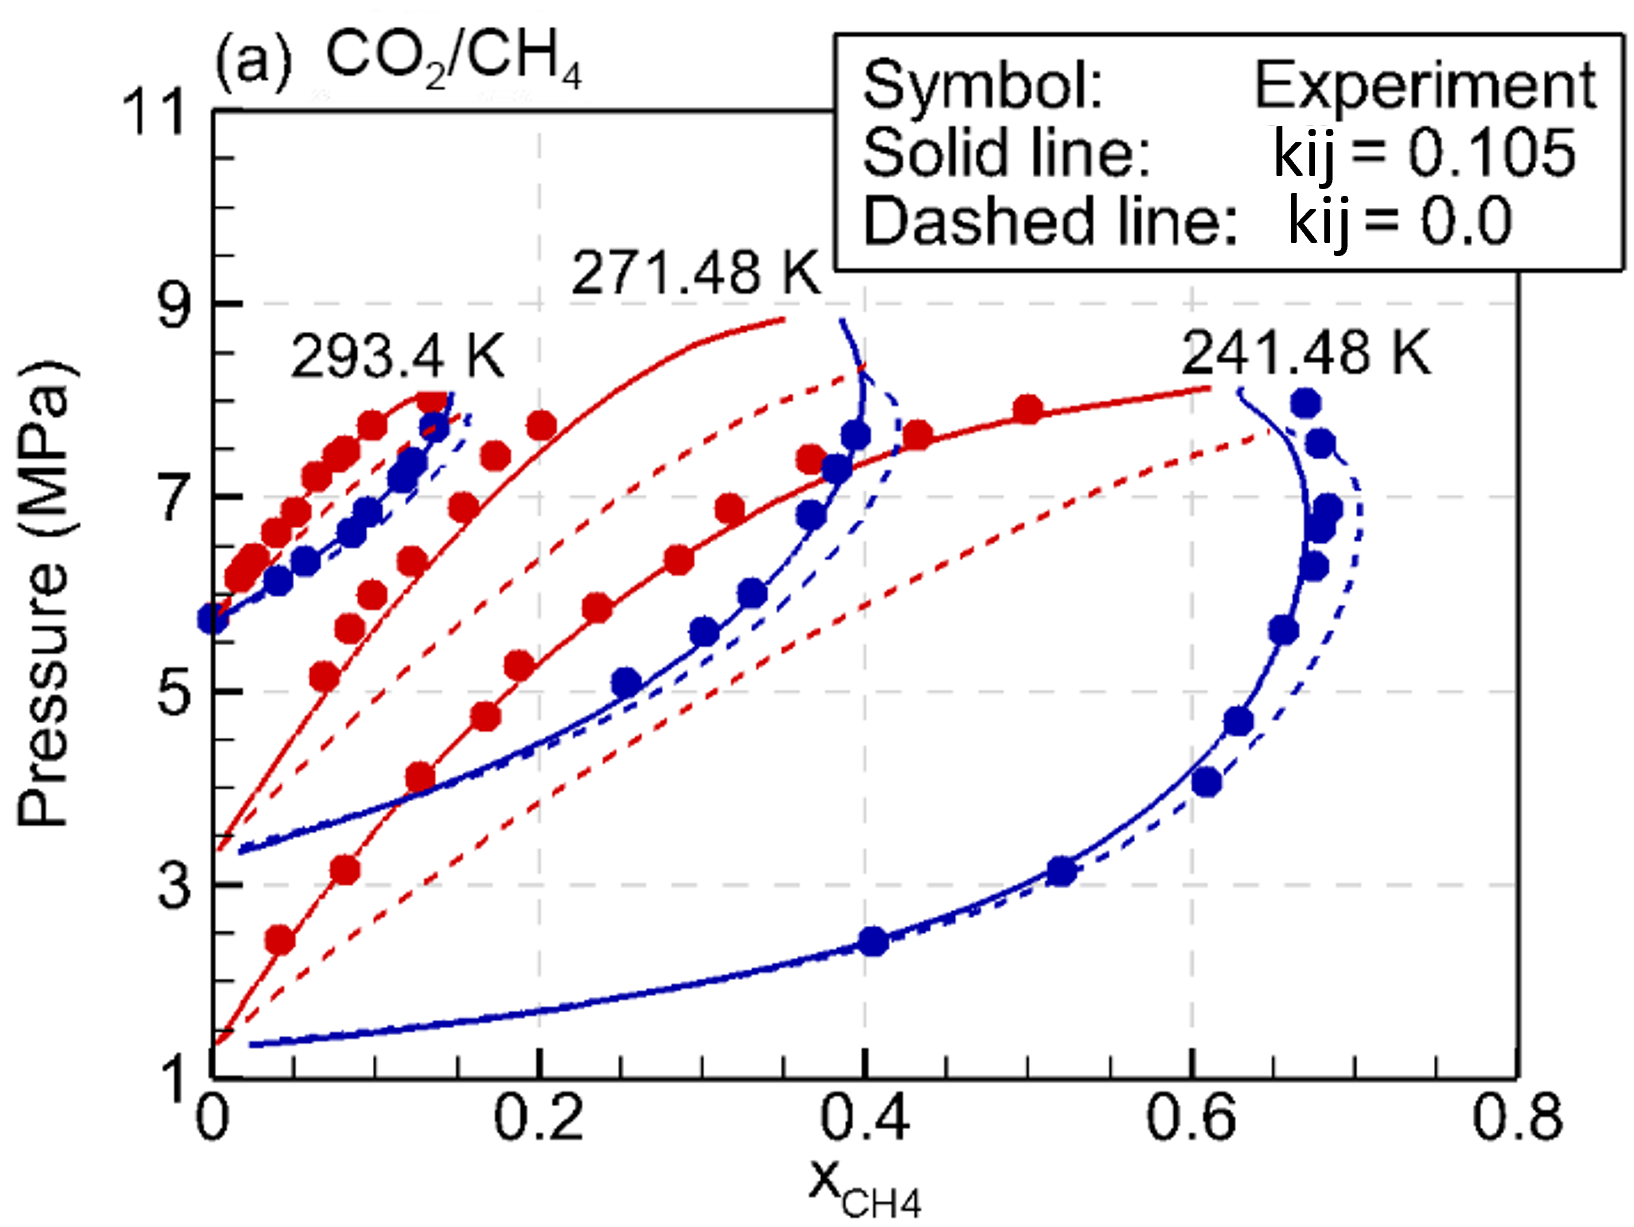
\includegraphics[width=0.5\linewidth]{phase_diagram_PX_CO2_CH4_2.png}
            %\caption{fig1}
            %\end{minipage}%
        }%
        \subfigure{
            %\begin{minipage}[t]{0.5\linewidth}
            \centering
            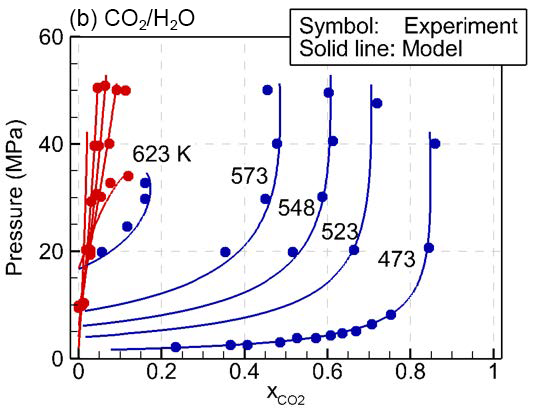
\includegraphics[width=0.5\linewidth]{phase_diagram_PX_CO2_H2O.png}
            %\caption{fig2}
            %\end{minipage}%
        }%
        \caption{Comparison of pressure-composition phase boundaries between experimental measurements and model predictions: (a) mixtures of \ce{CO2} and \ce{CH4}; (b) mixtures of \ce{CO2} and \ce{H2O}. Symbol: experimental data \cite{somait1978liquid}; line: model prediction. In sub-figure (a), solid line: binary interaction parameter $k_{ij}=0.105$ is used; dashed line: $k_{ij}=0$ is used. In sub-figure (b), binary interaction parameter $k_{ij}=0.137$ is used. Red color: bubble points/curve, blue color: dew points/curve.}
        \label{v1}
    \end{figure}

Because in this study we are also dealing with mixtures of \ce{N2}, \ce{n-C8H18}, and \ce{n-C12H26}. We extended our validation to include VLE calculations for N2 when mixed separately with the aforementioned substances, as illustrated in Fig.~\ref{C8_vali} and Fig.~\ref{C12_vali}. The binary interaction parameters used in these calculations were sourced from references \cite{eliosa2009vapor,garcia2011vapor}. The results, as depicted, demonstrate good accuracy in predicting VLE within the temperature range of approximately 300K-600K. However, it is worth noting that as pressure levels increase beyond a certain threshold, a slight deviation in the prediction of phase boundaries becomes evident. This deviation can be attributed to the inherent limitations of the PREOS. Nevertheless, these predictions, while not perfect in the some regime, still suffice to provide a valuable qualitative analysis model, especially in scenarios involving transcritical flow.


%The TP flash solver is validated by comparing the predictions with the experimental data of Somait and Kidnay [5] in terms of the phase boundaries of CO2/CH4 and CO2/H2O mixtures. As shown in Fig. 3.1, the model prediction agrees with the experimental data very well for both mixtures. In Fig. 3.1 (a), we tested two different binary interaction parameters kij. As you can see, the difference in binary interaction parameters changes the phase boundary. Appropriate values can improve the accuracy of phase boundary prediction. Because in this study we are also dealing with mixtures of N2, n-C8H18, and n-C12H26. We also tested the VLE calculation of N2 mixed separately with two substances (see in Fig. 3.2 and Fig. 3.3). The selection of binary interaction parameters are from [7, 80]. It can be seen that the predictions of the VLE model are relatively accurate when compared with experimental results in the range of about 300K-600K. When the pressure continues to increase, prediction error of phase boundary emerges, which is caused by the limitations of the PREOS. However, it is enough to provide a good qualitative analysis model for transcritical flow.
    \begin{figure}[htbp]
        \centering
        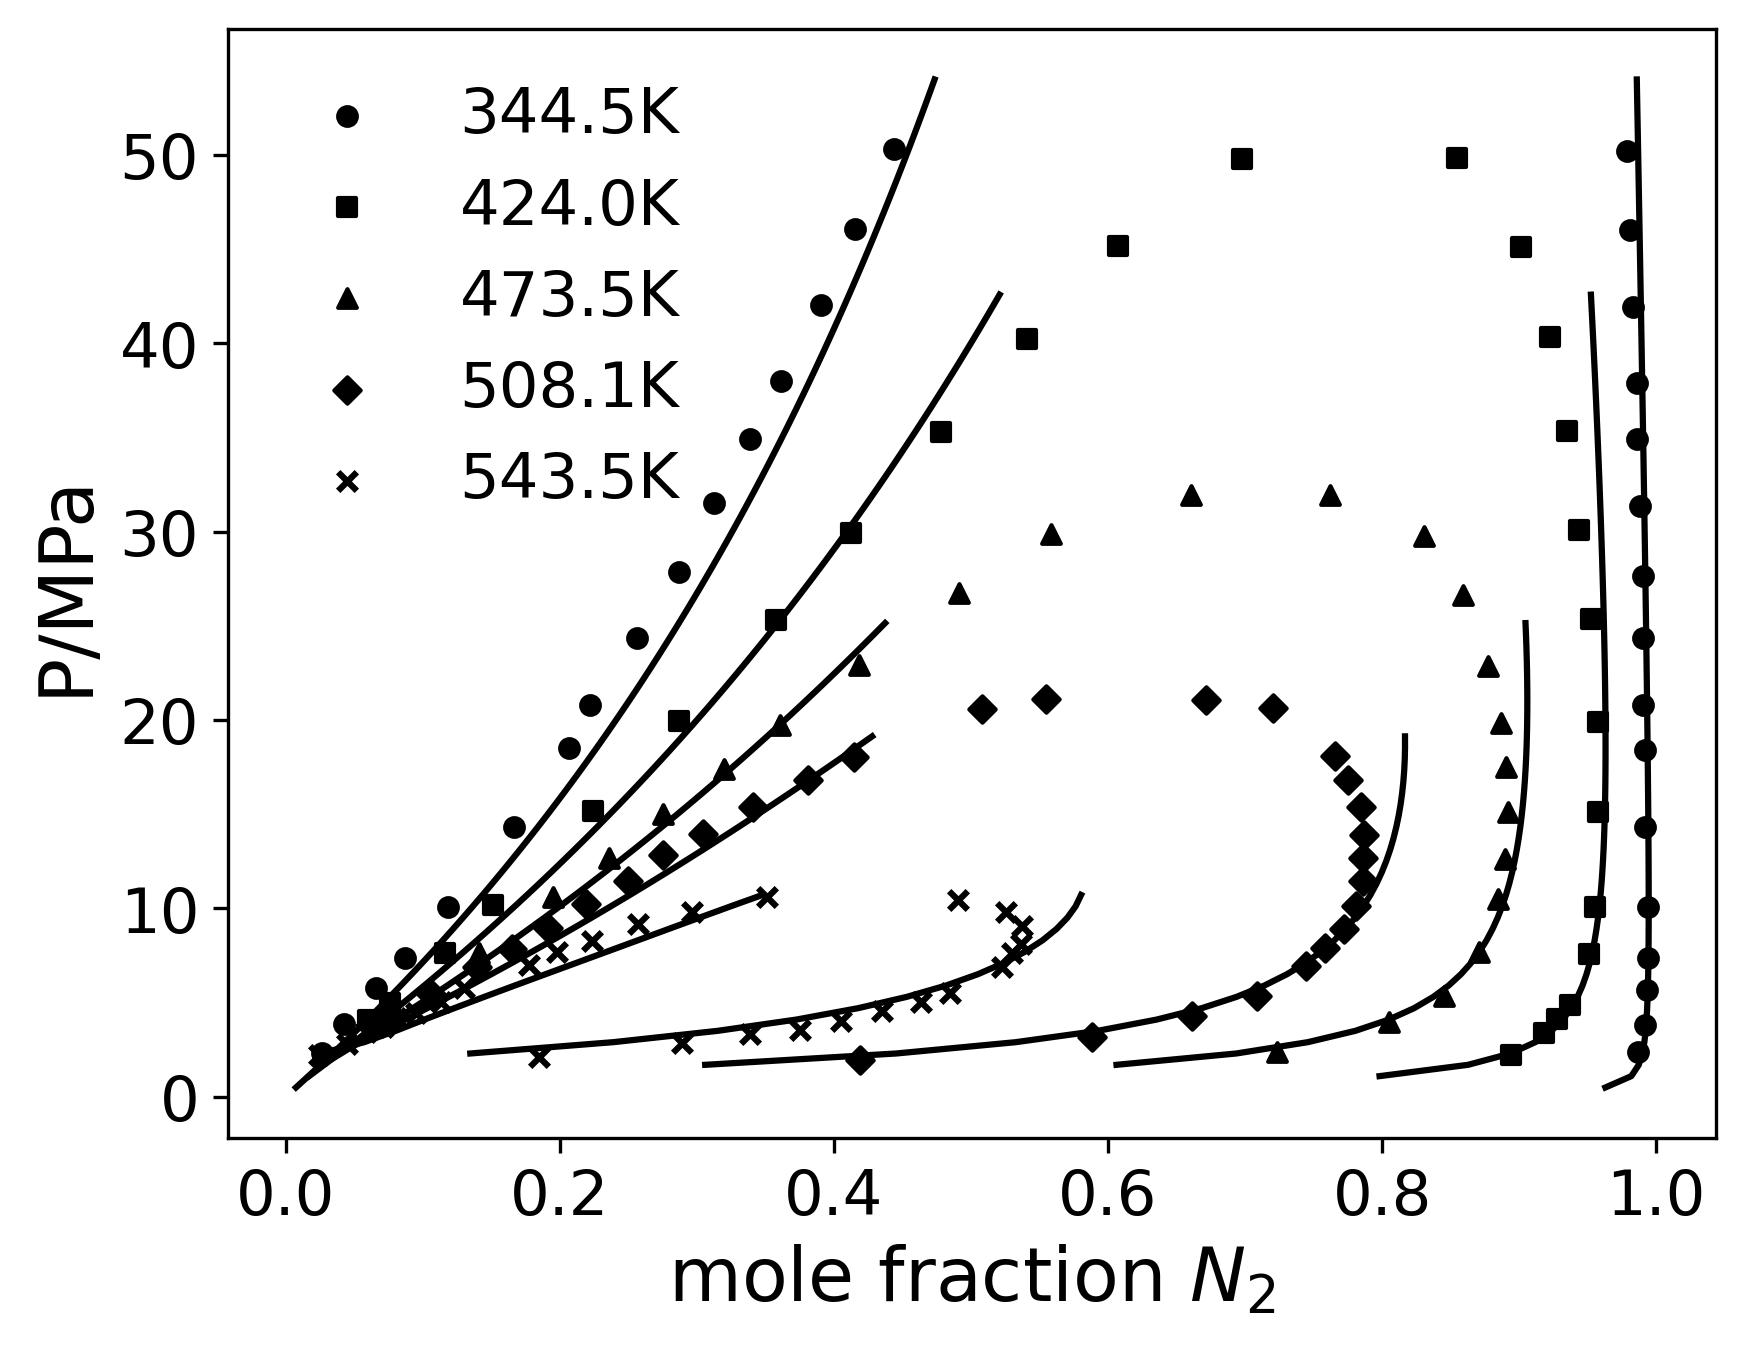
\includegraphics[width=0.7\linewidth]{C8_vali_paper.png}
        \centering
        \caption{Comparison of pressure-composition phase boundaries between experimental measurements and model predictions (mixture of \ce{N2} and \ce{n-C8H18}). Symbol: experimental data \cite{llave1988vapor}; line: model prediction. Binary interaction parameter $k_{ij}=0.1396$ is used.}
        \label{C8_vali}
    \end{figure}

    \begin{figure}[htbp]
        \centering
        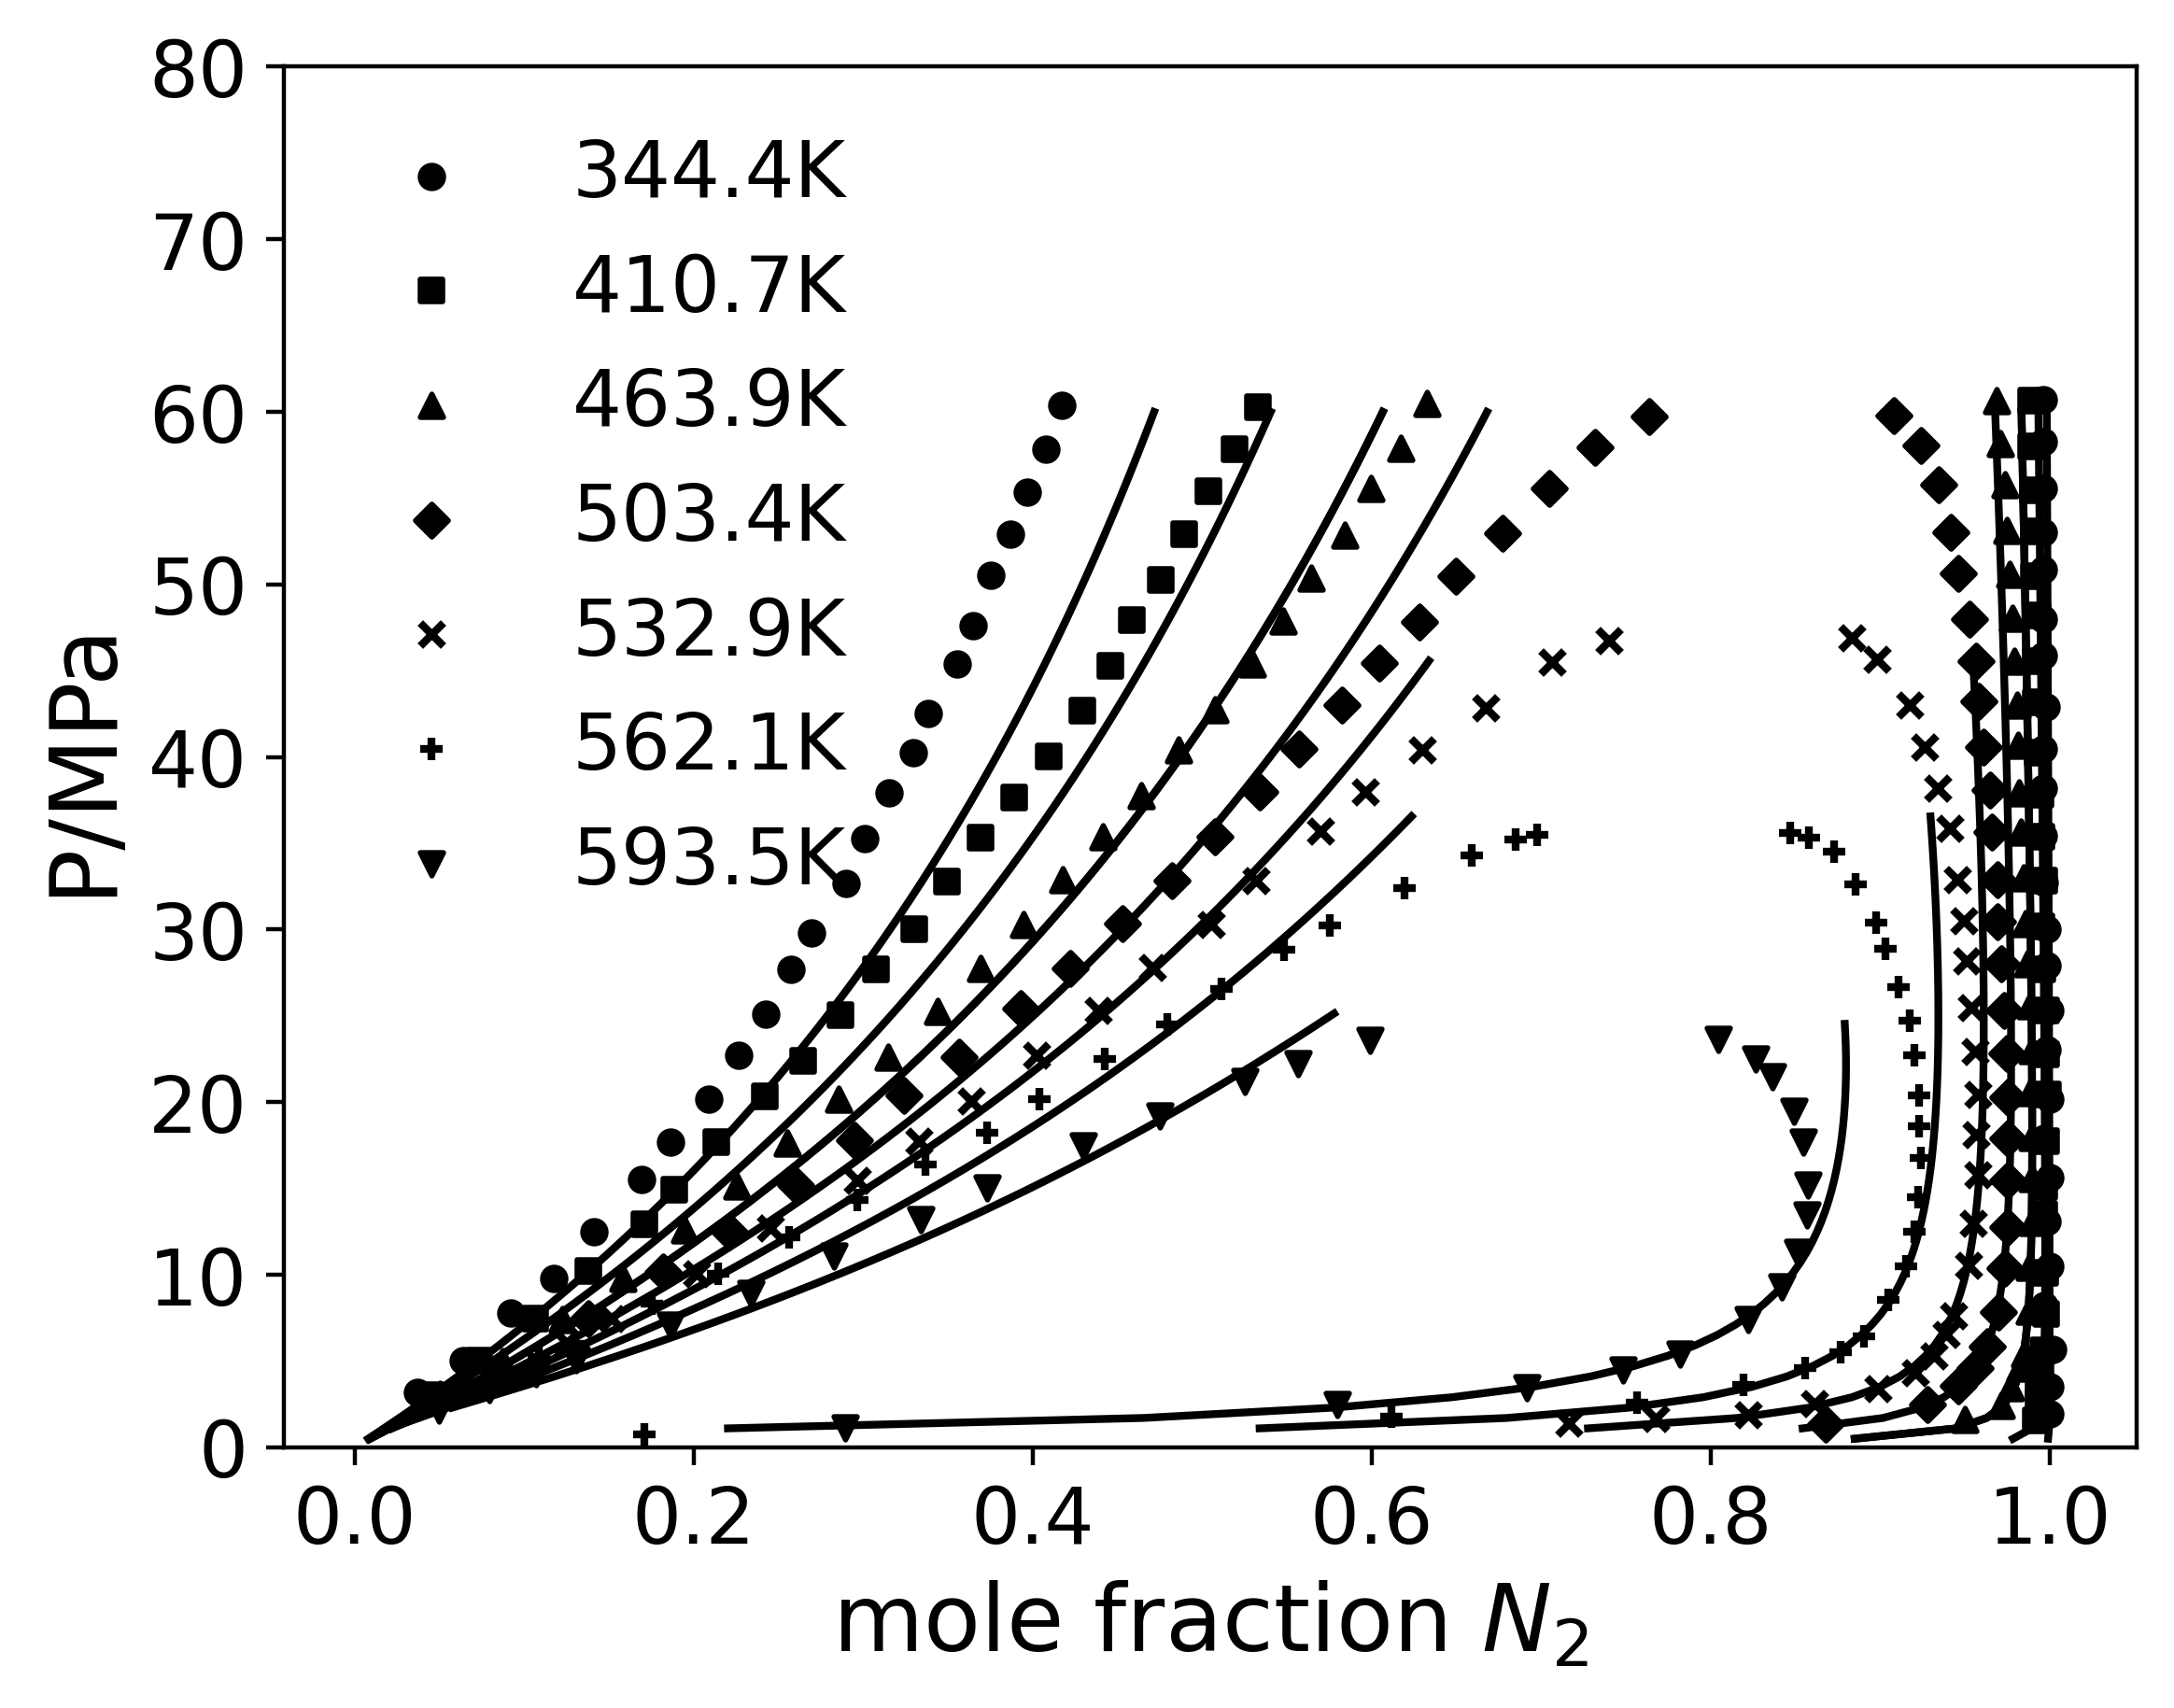
\includegraphics[width=0.7\linewidth]{C12_vali_paper.png}
        \centering
        \caption{Comparison of pressure-composition phase boundaries between experimental measurements and model predictions (mixture of \ce{N2} and \ce{n-C12H26}). Symbol: experimental data \cite{garcia2011vapor}; line: model prediction. Binary interaction parameter $k_{ij}=0.1561$ is used.}
        \label{C12_vali}
    \end{figure}

    
    \subsection{Verification of the TP flash solver based on mixture critical points}

    Next, we proceed to a comparative analysis of mixture critical points obtained through our VLE method, specifically utilizing the TP flash solver, with critical points derived from other methods. Within the VLE-based approach, critical points can be directly ascertained by identifying the intersection of the dew curve and the bubble curve.
    %%Next, the mixture critical points obtained from the VLE method (specifically, the TP flash solver) are compared with those obtained from several other methods. In the VLE-based method, critical points can be obtained directly from the intersection of the dew curve and bubble curve.
    Stradi et al. \cite{stradi2001reliable} introduced a critical point determination approach, drawing upon Heidemann and Khalil's criticality formulation \cite{heidemann1980calculation}, which has garnered widespread adoption due to its clear theoretical foundation. For a mixture of $C$ components,

   %% Stradi et al. \cite{stradi2001reliable} derived the mixture critical point based on Heidemann and Khalil's criticality formulation \cite{heidemann1980calculation} as below, which has been widely used due to its clear theoretical foundation. For a mixture of $C$ components,
    \begin{align}
         & Q\Delta \mathbf n=\mathbf0                                                                          \\
         & Q_{ij}=\left( \frac{\partial^2A}{\partial n_i \partial n_j}\right)_{T,V}                            \\
         & \sum_i^{C}\sum_{j}^{C}\sum_{k}^{C}A_{ijk}\Delta n_i\Delta n_{j}\Delta n_{k}=0                       \\
         & \Delta \mathbf n^{T}\Delta \mathbf n=1                                                              \\
         & A_{ijk}=\left( \frac{\partial^3A}{\partial n_i \partial n_j\partial n_k}\right)_{T,V} \label{eq:19}
    \end{align}
    where $\Delta \mathbf n$ means the nonzero perturbation vector of the component mole numbers; $A$ is the Helmholtz free energy. Notably, the Helmholtz free energy's reliance on the mixture composition implies that this method inherently hinges on the local mixture characteristics.
    %Since the Helmholtz free energy depends on the mixture composition, this way is implicitly dependent on the local mixture. 

In Harstad and Bellan's work \cite{harstad2004mixing}, a formulation of mixture critcal point is also provide:
      \begin{align}
         & T_{c,ij}=(1-k_{ij})\sqrt{T_{c,i}T_{c,j}}  \\
         & V_{c,ij}= \left(V_{c,i}^{1/3}+V_{c,j}^{1/3}\right)^3/8 \\
         & Z_{c,ij}=\left(Z_{c,i}+Z_{c,j}\right)/2   \\
         & P_{c,ij}= \frac{Z_{c,ij}RT_{c,ij}}{V_{c,ij}} 
    \end{align}
where subscript ``$c,ij$'' is the mixture critcal property, and subscript ``$c,i$'' the critcal property of component $i$.
    
    
    The binary critical points predicted by the above methods are compared in Fig.~\ref{v2_new}, and the predictions of the current VLE-based method agree very well with Stradi et al.'s formulation \cite{stradi2001reliable} for the mixture of \ce{CH4} and \ce{H2S}, while VLE's prediction are quite different from the results using Harstad and Bellan's method. This is because their method is not designed to capture changes in the composition of the mixture, which VLE and Stradi et al.'s methods are capable of. But note that Stradi et al.'s formulation can only predict critical points, and it cannot provide other detailed information (e.g., phase boundaries) about phase diagrams like what VLE solver can provide.


 %   \begin{figure}[htbp]
 %       \begin{center}
 %           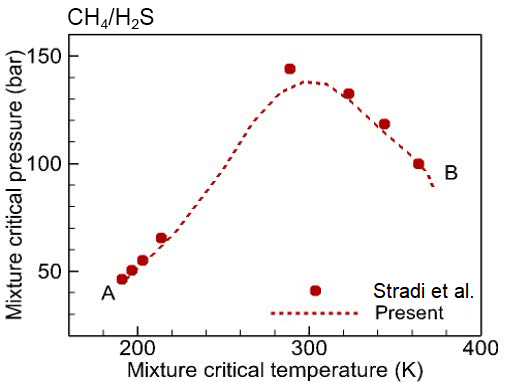
\includegraphics[width=0.55\linewidth]{critical_point_CH4_H2S.png}
            %\includegraphics[width=0.45\linewidth]{thermal/vali2_v2.png}
 %       \end{center}
 %       \caption{Comparison of predicted mixture critical points of \ce{CH4}/\ce{H2S} mixtures between Stradi et al. \cite{stradi2001reliable} and the present work (overall mole fraction of \ce{CH4} is increased from 0.01 at A to 0.99 at B).
%        }
%        \label{v2}
%    \end{figure}

    \begin{figure}[htbp]
        \begin{center}
            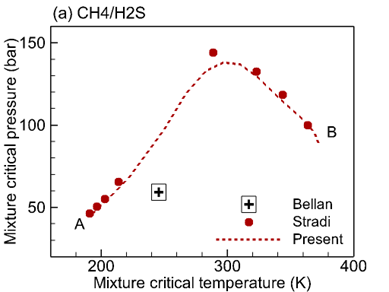
\includegraphics[width=0.45\linewidth]{critical_point_CH4_H2S_new.png}
            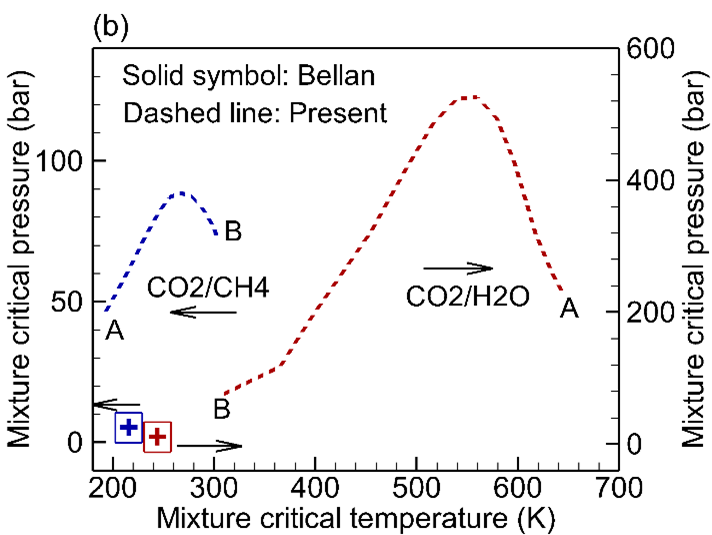
\includegraphics[width=0.45\linewidth]{critical_point_2.png}
            %\includegraphics[width=0.45\linewidth]{thermal/vali2_v2.png}
        \end{center}
        \caption{Comparison of predicted mixture critical points (a) comparison for the mixture of \ce{CH4}/\ce{H2S} between Harstad and Bellan \cite{harstad2004mixing}, Stradi et al., \cite{stradi2001reliable} and present work, the mole fraction of \ce{CH4} is increased from 0.01 to 0.99 from A to B; (b) comparison for the mixture of \ce{CO2}/\ce{CH4} and \ce{CO2}/\ce{H2O}, the mole fraction of \ce{CO2} is increased from 0.01 to 0.99 from A to B.}
        \label{v2_new}
    \end{figure}

    \subsection{Verification of PH flash solver based on equilibrium mixing temperature $T_{eq}$}
 Here, the HPn flash solver is verified by the Fig.~\ref{v6} in Matheis and Hickel \cite{matheis2018multi}. In this case, we mix 900K \ce{N2} with 363K \ce{n-C12H26} at 6MPa, assuming constant enthalpy. In the work of Matheis and Hickel\cite{matheis2018multi}, VLE was also used for prediction, so we can verify our implementation. As shown in Fig.~\ref{v6},our current predictions of equilibrium mixing temperature $T_{eq}$ exhibit a good agreement with the outcomes reported by Matheis and Hickel, further affirming the accuracy and reliability of our PH flash solver.

    \begin{figure}[htb]
        \begin{center}
            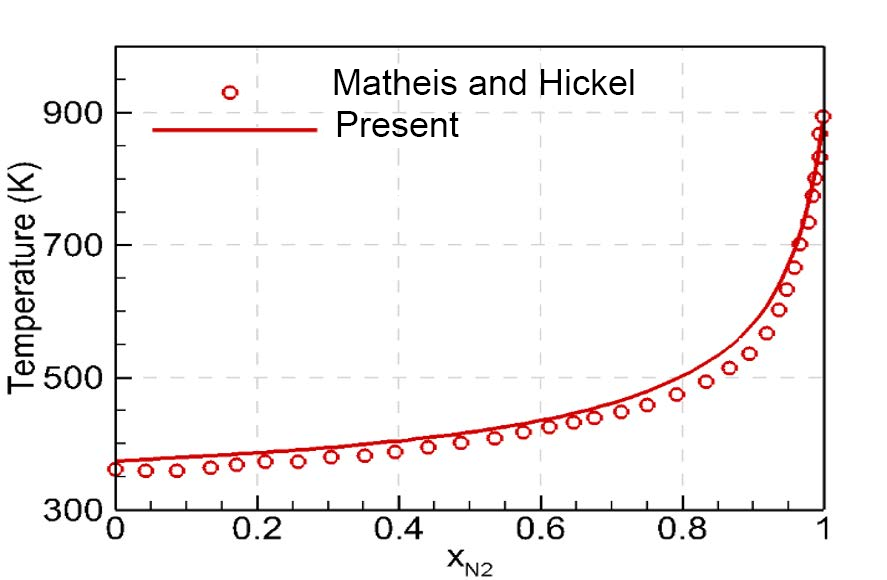
\includegraphics[width=0.7\linewidth]{mixing_temperature_C12_N2.png}
        \end{center}
        \caption{Comparison of predicted equilibrium mixing temperatures $T_{eq}$ for \ce{n-C12H26}/\ce{N2} mixtures between Matheis and Hickel \cite{matheis2018multi} and the current model.}
        \label{v6}
    \end{figure}

    \subsection{Validation and verification of the CFD solver} \label{App:vali:CFD}
    %%Since the pressure-based solver is mainly used for low Mach flow simulation. We want to test the PIMPLE solver further before using it for compressible flow simulations. Two 1D shock tube simulations are conducted to validate and verify the pressure-based CFD solver. First, Sod shock tube \cite{sod1978survey} is used to test the CFD solver with the ideal gas model, and the results are shown in Fig.~\ref{vali1ST}. The pressure and temperature evolution show a good agreement with the exact solution. Although the PIMPLE algorithm is majorly used for low Mach flow, the 1D Sod shock tube results clearly show that this compressible version of PIMPLE algorithm can well capture the shock wave and accurately predict compressible flows. Moreover, the results show that the scheme is not dissipative, as the sharp gradients (e.g., near the shock) are accurately captured with only 200 grid cells and there is no spurious oscillation near the high gradients. Second, results from a shock tube simulation with phase change are compared with Chiapolino et al.'s simulation results \cite{chiapolino2017simple}, as shown in Fig.~\ref{vali2ST}. The shock tube is filled with a homogeneous water-air mixture, and the initial discontinuity is located at 0.5 m. Chiapolino et al.'s model used the Noble Abel Stiffened Gas (NASG) EOS and also assumed mechanical and thermodynamic equilibrium. Therefore, their results can also capture the phase change in the shock tube, which is valuable as a reference to verify the implementation of the VLE-based CFD simulation framework in this study both qualitatively and quantitatively. Good agreements were obtained in terms of the evolution of pressure and temperature at the contact discontinuity.
As the pressure-based solver is primarily used for low Mach flow simulations, our objective is to assess the performance of the PIMPLE solver before deploying it for compressible flow simulations. To achieve this, we conducted two 1D shock tube simulations, aiming to validate and corroborate the capabilities of the pressure-based CFD solver.

The first simulation involved the Sod shock tube \cite{sod1978survey} to test the CFD solver using the ideal gas model. The results, depicted in Fig.~\ref{vali1ST}, exhibit remarkable agreement with the exact solution. Despite the PIMPLE algorithm's typical usage in low Mach flow scenarios, the outcomes of the 1D Sod shock tube simulation unequivocally demonstrate its competence in accurately capturing shock waves and predicting compressible flows. Furthermore, these results affirm that the scheme is non-dissipative, as evidenced by its accurate representation of sharp gradients, especially in the vicinity of the shock, with just 200 grid cells and the absence of spurious oscillations near high gradients.


%Note that Chiapolino et al. used a fully compressible CFD solver (based on MUSCL Hancock method using van Leer’s slope limiter and HLLC Riemann solver), while the CFD solver in this study uses a pressure-based PIMPLE method (which can be called a ``low-Mach'' solver but was extended to a transonic version). For this reason, the fact that both CFD solvers agree with each other can imply that the observed discrepancy between the CFD results with and without phase change (i.e., with and without VLE) in Fig.~\ref{v9} should not come from numerical implementation but should come from the real physics of the shock tube problem.
    \begin{figure}[htbp]

            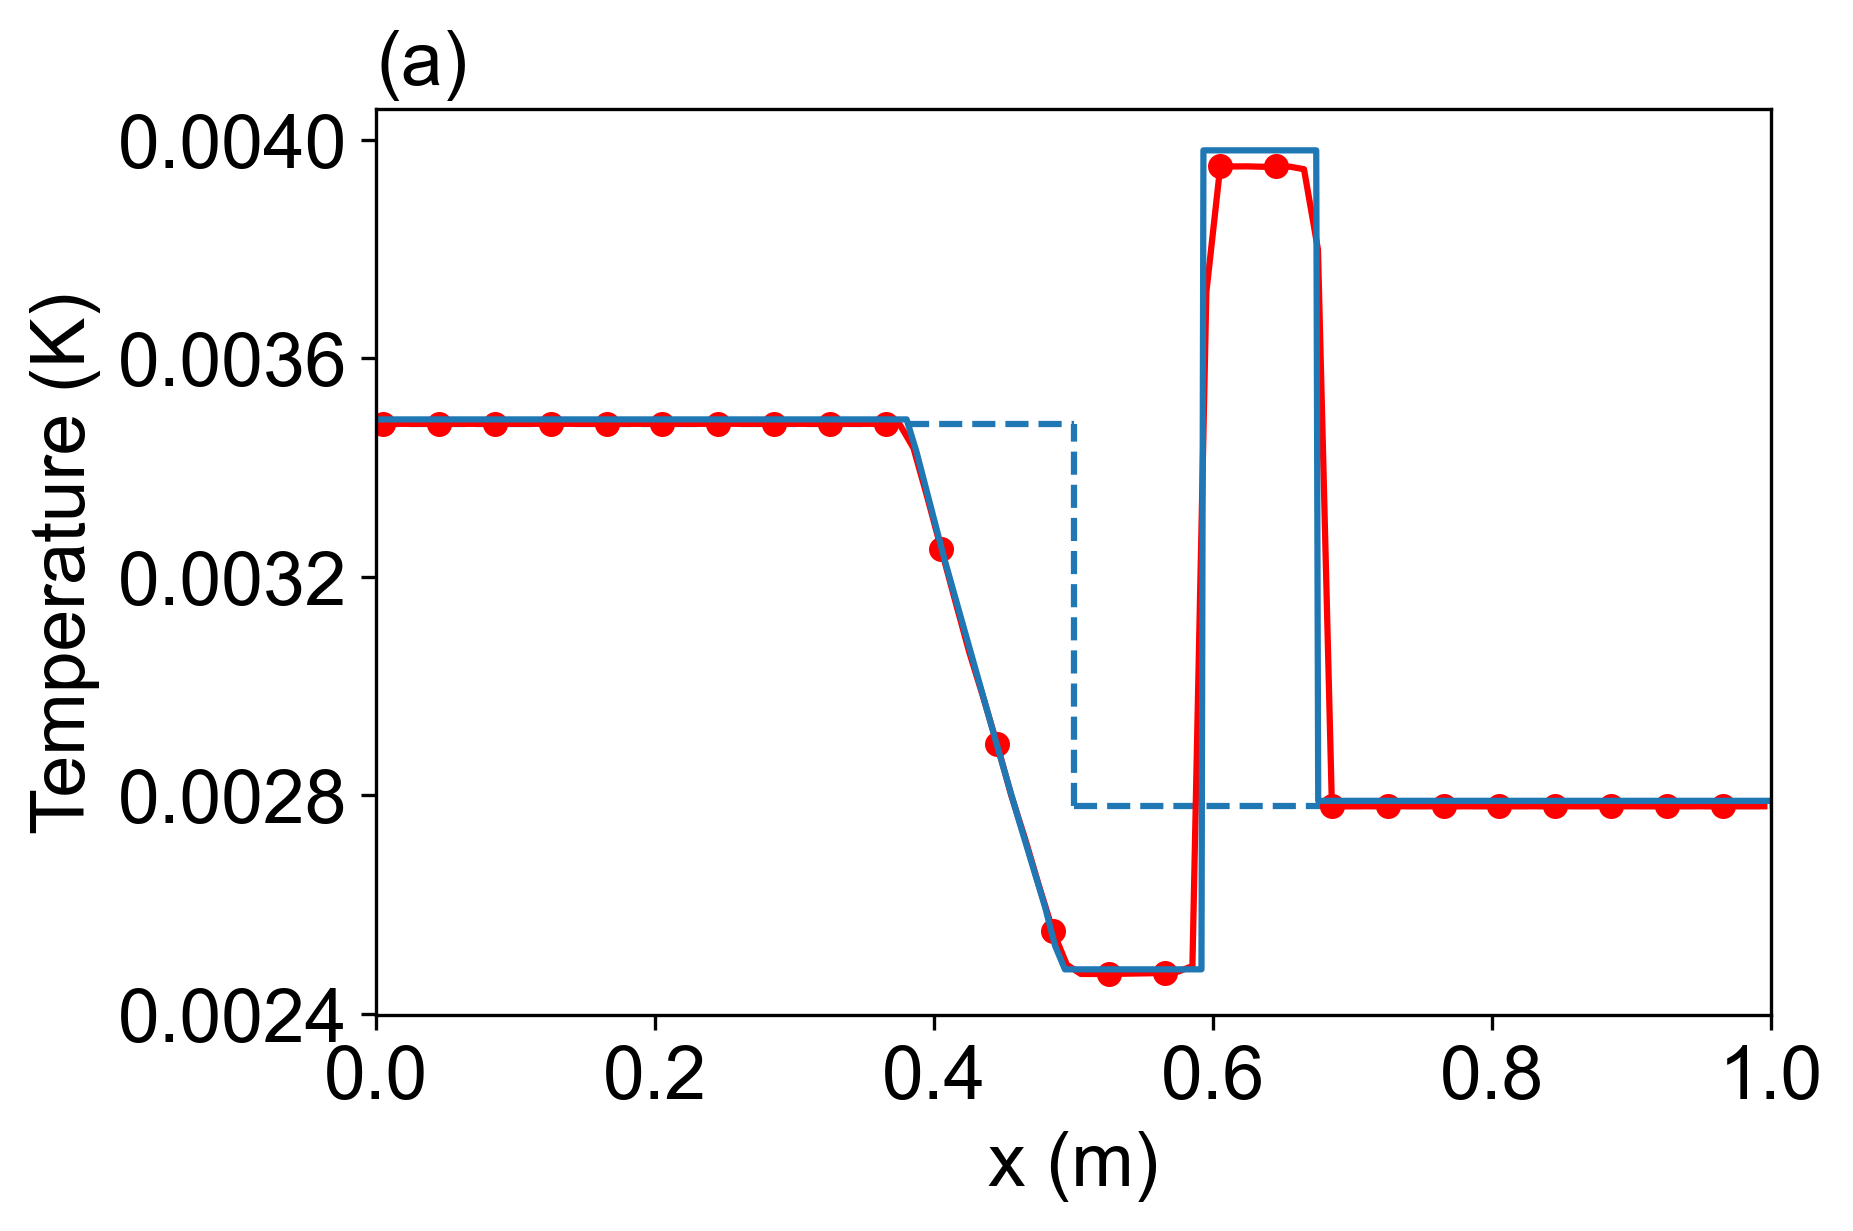
\includegraphics[width=0.465\linewidth]{sodT_v2.png}
            \includegraphics[width=0.435\linewidth]{sodP_V2.png}

        \caption{Validation of the VLE-based CFD solver by Sod shock tube simulations \cite{sod1978survey}. Initial conditions: $P_{\rm{left}} = 1$ Pa, $P_{\rm{right}} = 0.1$ Pa, $T_{\rm{left}} = 0.00348$ K, $T_{\rm{right}} = 0.00278$ K, the initial discontinuity is at $x=0.5$ m; fluid: air; $t=0.1$ s; 200 grid cells, CFL = 0.2.}
        \label{vali1ST}
    \end{figure}
    
In the second simulation, we compared the results of a shock tube simulation with phase change to Chiapolino et al.'s works \cite{chiapolino2017simple}, as illustrated in Fig.~\ref{vali2ST}. This shock tube contained a homogeneous water-air mixture, with the initial discontinuity positioned at 0.5 m. Chiapolino et al. employed the Noble Abel Stiffened Gas (NASG) equation of state and assumed both mechanical and thermodynamic equilibrium in their model. Chiapolino et al. used a fully compressible CFD solver based on MUSCL Hancock method using van Leer’s slope limiter and HLLC Riemann solver. Consequently, their results aptly captured the phase change within the shock tube, serving as a valuable reference for validating our implementation of the VLE-based CFD simulation framework. We achieved good agreement in terms of pressure and temperature evolution at the contact discontinuity, both qualitatively and quantitatively.

     \begin{figure}[htbp]

        \centering

            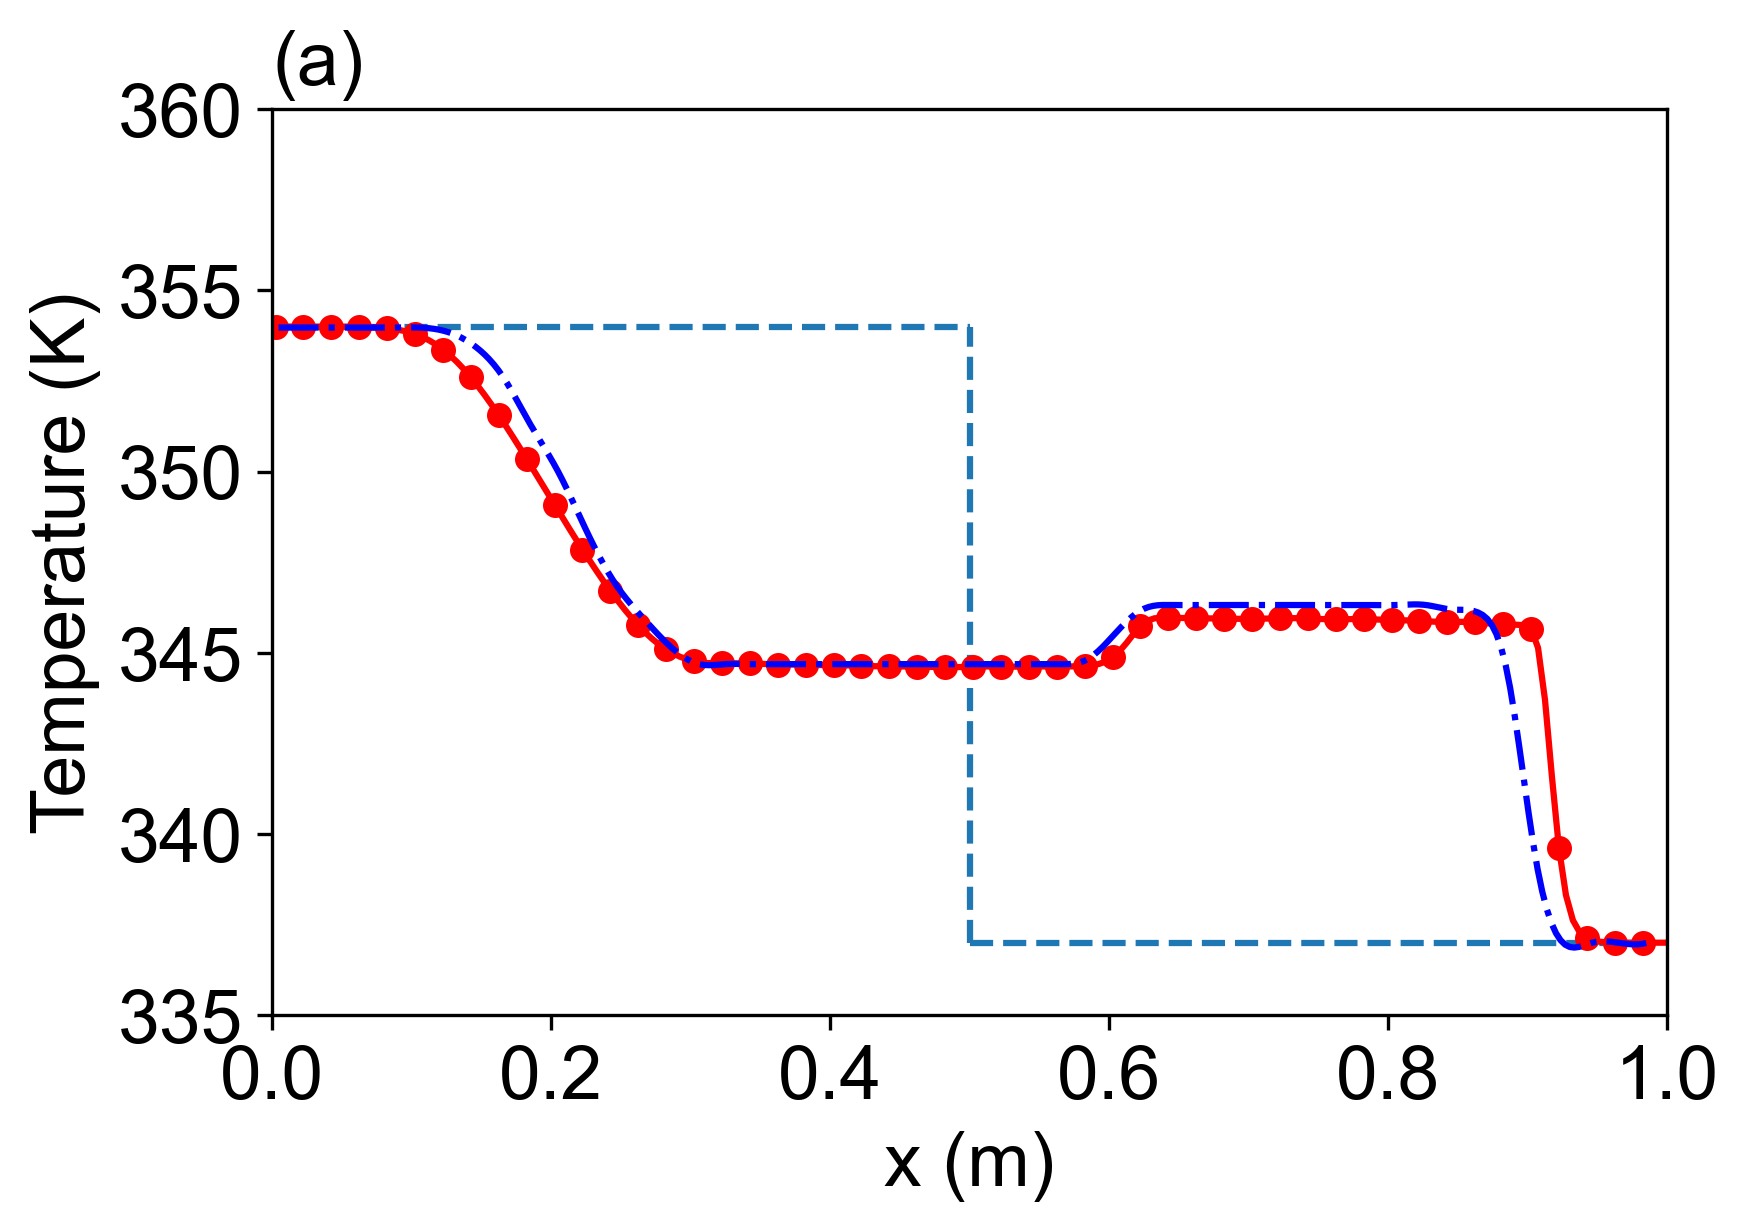
\includegraphics[width=0.45\linewidth]{valiT_v2.png}
            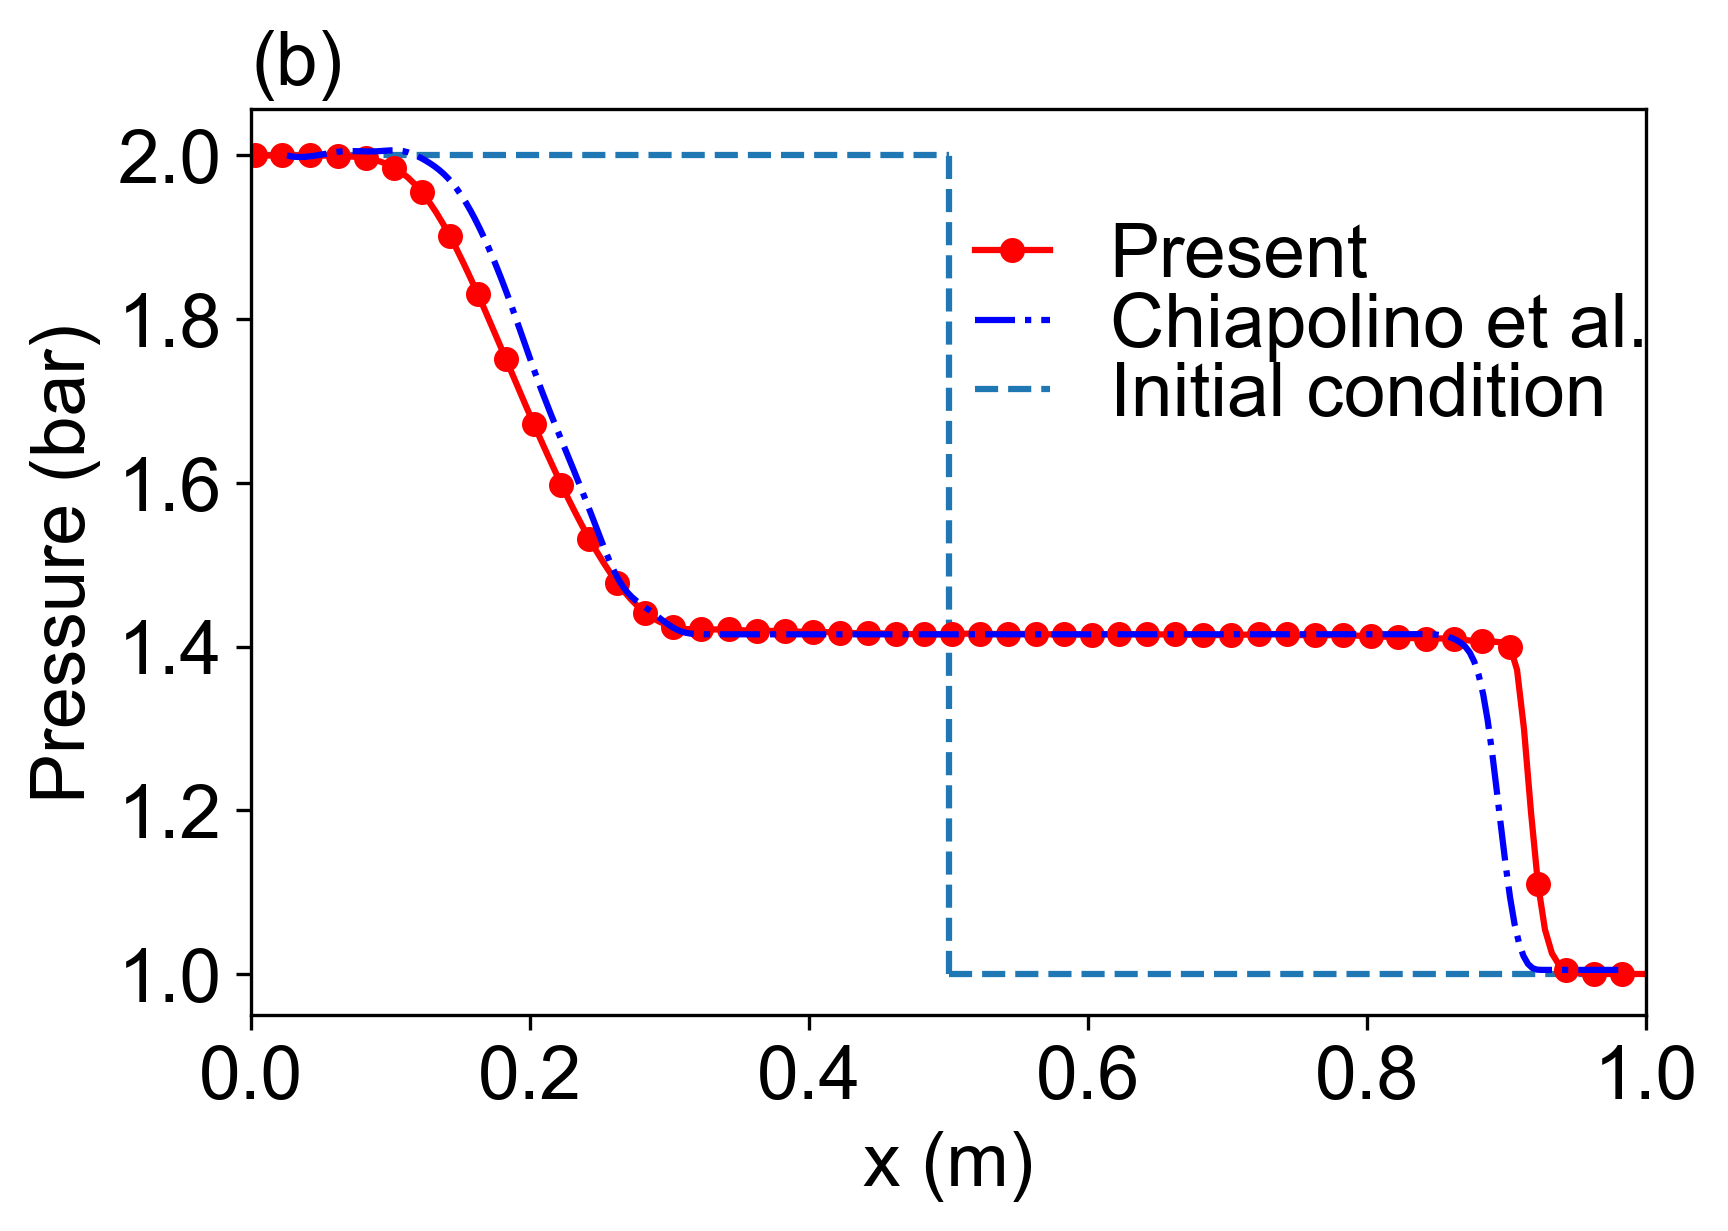
\includegraphics[width=0.45\linewidth]{valiP_v2.png}
        \caption{Verification of the VLE-based CFD solver by Chiapolino et al.'s shock tube simulations  \cite{chiapolino2017simple}. Initial condition: $P_{\rm{left}} = 2$ bar, $P_{\rm{right}} = 1$ bar, $T_{\rm{left}} = 354$ K, $T_{\rm{right}} = 337$ K, $Y_{\rm{H_2O,\ left}} = Y_{\rm{H_2O,\ left}} = 0.3$, $Y_{\rm{Air,\ left}} = Y_{\rm{Air,\ left}} = 0.7$; $t = 1.0$ ms, 200 grid cells, CFL = 0.1, the initial discontinuity is at $x=0.5$ m.}
        \label{vali2ST}
    \end{figure}
\comment{
    LES of a jet-in-crossflow is also conducted to validate the CFD solver. The results are compared with Su and Mungal's experimental data \cite{su2004simultaneous}. The experiments were performed in an updraft wind tunnel with air as the crossflow fluid and nitrogen as the jet fluid. The crossflow and nitrogen are both at 300 K and 1 atm. Nitrogen is seeded with acetone vapor to 10\% by volume for diagnostic purposes, which is also considered in the simulation. The tunnel crossflow velocity profile has a peak value of $v_{\infty}=2.95\ \rm{m/s}$. Nitrogen is injected from a nozzle with inner diameter $d=4.53\ \rm{mm}$, the jet average velocity is $u_0=16.9\ \rm{m/s}$. The mesh in the simulation contains 1.3M cells in total, and the average cell size is 2.3 mm. A finer mesh ($500\ \rm{\mu m}$) is used to capture the detailed flow structure near the injection nozzle. Based on the binary diffusivity of acetone and air ($D=0.104\ \rm{cm}^2\rm{s}^{-1}$) and the kinematic viscosity of air ($\nu=0.155\ \rm{cm}^2\rm{s}^{-1}$), Schmidt number, $Sc\equiv \nu/D$, of the system is 1.49. In Fig.~\ref{valiJIC}, the center streamline and \ce{N2} centerline of time-averaged field are compared between the simulation and experiments. The center streamline is the streamline that goes through the center of injector, and the \ce{N2} centerline is the line of maximum \ce{N2} concentration points at fixed-y planes. Length scales are properly normalized by the factor $rd$, where $d$ is the jet diameter (4.53 mm), $r$ is ratio of jet velocity to crossflow velocity: $r\equiv u_0/v_{\infty}=5.7$. The simulation results agree well with the experimental data at $x>2rd$, but show a small deviation near the injection nozzle.
    This validation indicates that our CFD solver and LES models can accurately predict the mixing process at least for ideal gas.

    \begin{figure}[htb]
        \begin{center}
            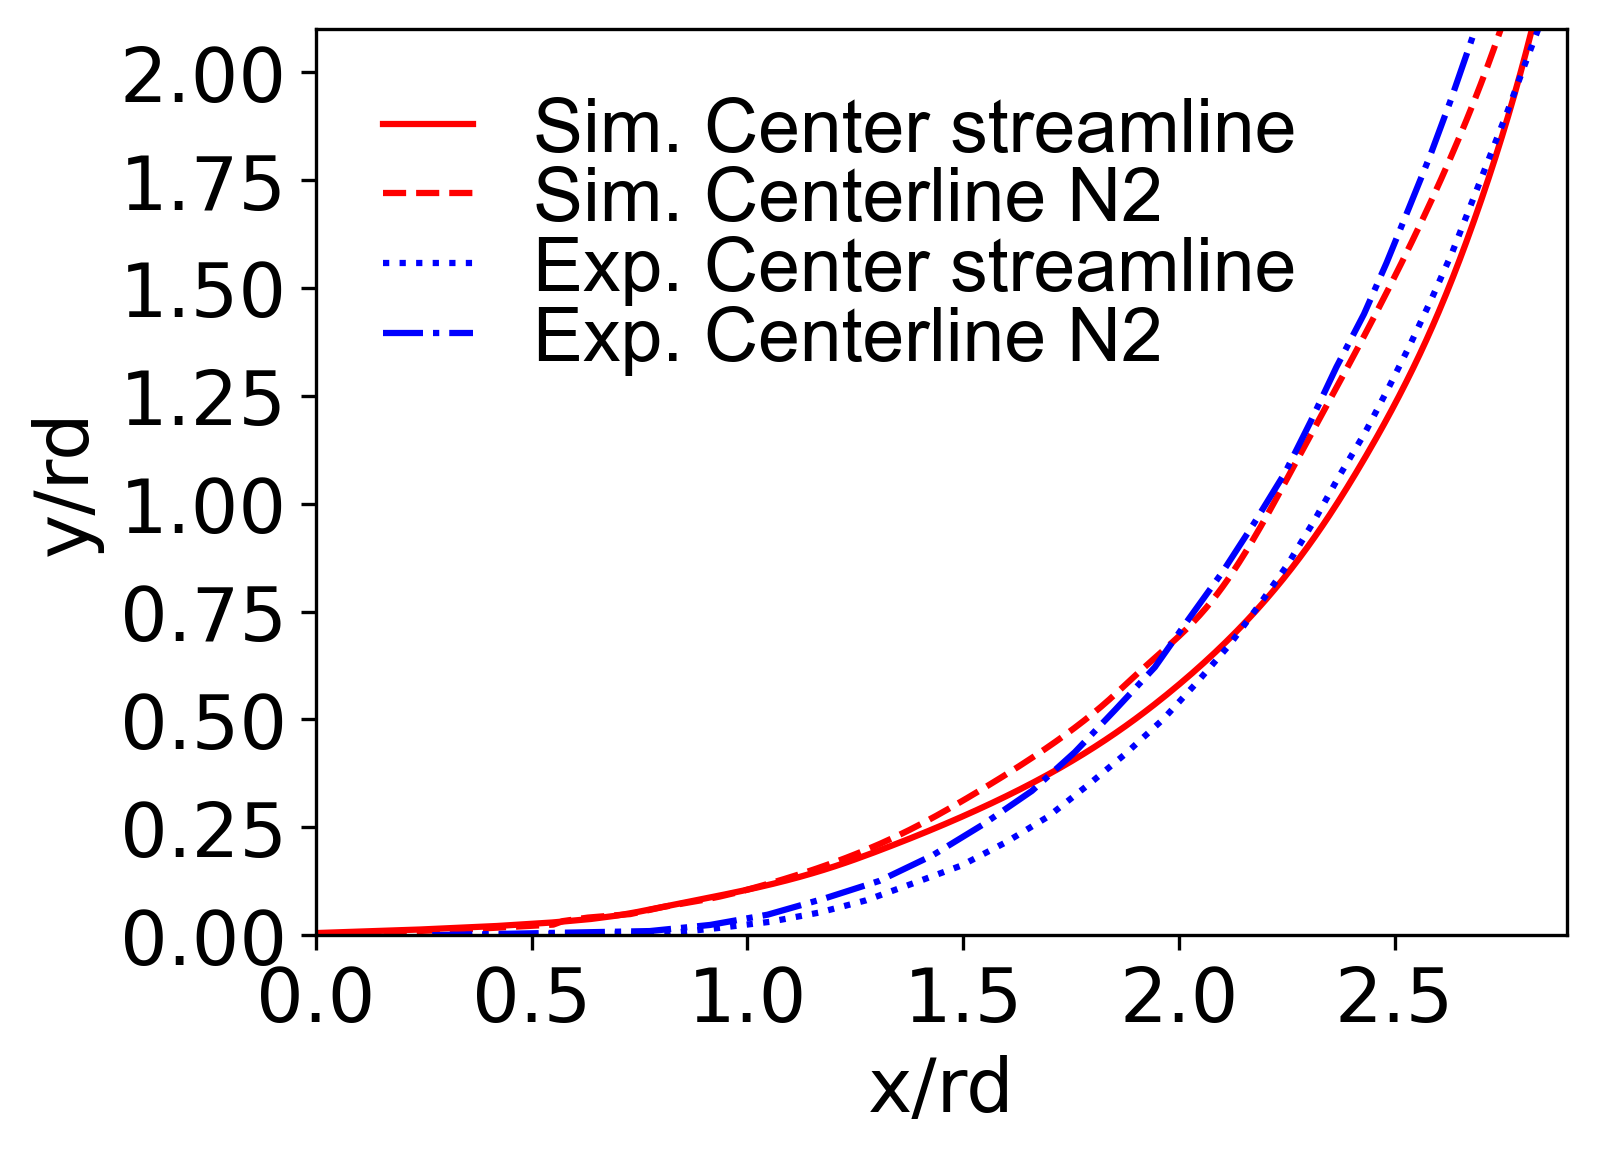
\includegraphics[width=0.5\linewidth]{valiJIC.png}
        \end{center}
        \caption{Comparison of a jet-in-crossflow between the present model prediction and experimental data \cite{su2004simultaneous}. Blue: experimental data; red: simulation prediction.}
        \label{valiJIC}
    \end{figure}
}








%%%%%%%%%%%%%%%%%%%%%%%%%%%%%%%%%%%%%%%%%%%%%%%%%%%%%%%%%%%%%%%%%%%%%%%%%%%%%%%%
